\documentclass[a4j,12pt,]{jarticle}
 \usepackage[dvipdfmx]{graphicx}
 \usepackage{float}
 \usepackage{siunitx} %%SI単位系用
 \usepackage{amssymb, amsmath}
 \usepackage{ascmac,here,txfonts,txfonts}
\usepackage{listings,jlisting}
\usepackage[dvipdfmx]{color}
\lstset{%
  language={Python},
  basicstyle={\small},%
  identifierstyle={\small},%
  commentstyle={\small\itshape\color[rgb]{0,0.5,0}},%
  keywordstyle={\small\bfseries\color[rgb]{0,0,1}},%
  ndkeywordstyle={\small},%
  stringstyle={\small\ttfamily\color[rgb]{1,0,1}},
  frame={tb},
  breaklines=true,
  columns=[l]{fullflexible},%
  numbers=left,%
  xrightmargin=0zw,%
  xleftmargin=3zw,%
  numberstyle={\scriptsize},%
  stepnumber=1,
  numbersep=1zw,%
  lineskip=-0.5ex%
}
\begin{document}

{\noindent\small 第8回報告書 \hfill\today}
\begin{center}
  {\Large 実測値の概形が相互相関の最大値の計算に与える影響の調査}
\end{center}
\begin{flushright}
  祖父江匠真 \\
\end{flushright}

\section{はじめに}
前回, 日時の間隔を均一になるよう線形補間した後に, 相互相関が最大となるラグの選定を行ったが, その結果, 実測値と計算値の日時を809 \si{\second}ずらした時に相互相関が最大となった.

これは, ElasticSearchサーバーに保存されているドキュメントのタイムスタンプの情報とPCSの計測日時との間にズレが生じているのか, それとも相互相関の計算結果が誤っているのかのどちらが原因となっているのか判断できなかったので, 今回は, 晴れの日の割合が多い期間の実測データと, 雨の日の割合が多い期間の実測データのそれぞれに対して, 相互相関が最大となるラグを求めることで, 実測データの概形と相互相関が最大となるラグの関係について調査する.

\section{相互相関に使用する実測データの選定}
相互相関の計算に使用する実測値の日射量データとして, 晴れの日の割合が大きい期間と, 雨の日の割合が大きい期間の2種類を選ぶ.
晴れの日の割合が大きい期間は, 2022年4月1日0時0分から2022年4月8日12時0分までの7.5日間, 雨の日の割合が大きい期間は, 2022年4月23日0時0分から2022年4月30日12時0分までの7.5日間とした.

図\ref{p1}に, 晴れの日の割合が大きい期間の実測データを示す.

\begin{figure}[H]
  \begin{center}
    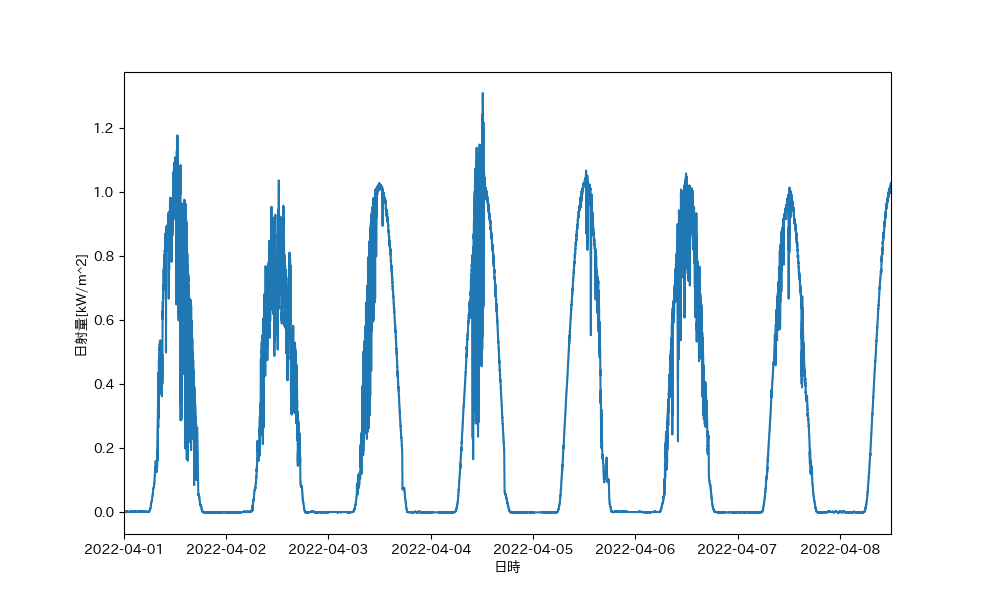
\includegraphics[width=160mm]{1.png}
    \caption{晴れの日の割合が大きい期間の実測データ}
    \label{p1}
  \end{center}
\end{figure}

図\ref{p2}に, 雨の日の割合が大きい期間の実測データを示す.

\begin{figure}[H]
  \begin{center}
    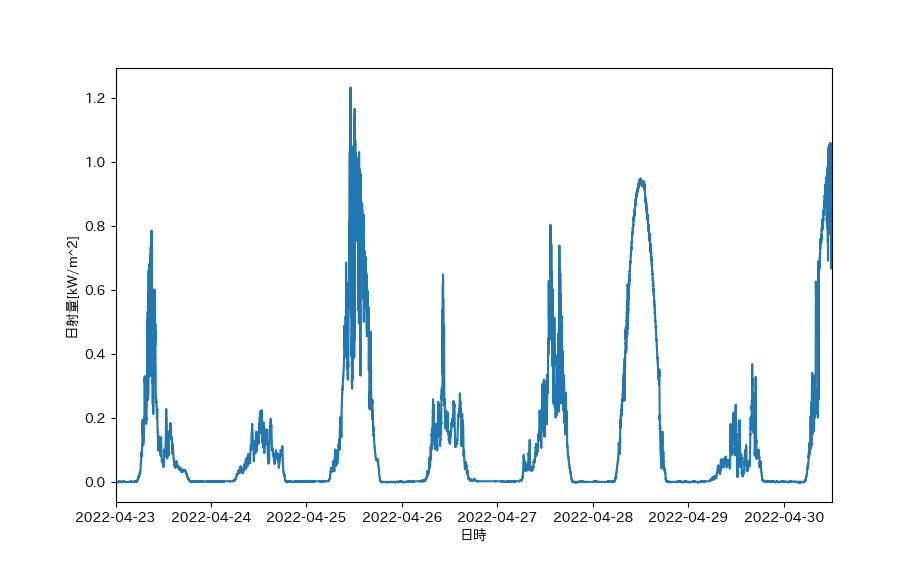
\includegraphics[width=160mm]{2.png}
    \caption{雨の日の割合が大きい期間の実測データ}
    \label{p2}
  \end{center}
\end{figure}

図\ref{p1}, 図\ref{p2}の実測データに対して, 計算値の日射量データの範囲を7日間として, 1分ずつスライドさせ, そのたびに実測値データとの相互相関を計算して, 相互相関が最大となるラグを求める.

相互相関を求めた結果, 図\ref{p1}では, 計算値の日時を実測値より32 \si{\second}進めた際に, 相互相関の値が最大となった.
また, 図\ref{p2}では, 計算値の日時を実測値より750 \si{\second}遅らせた際に, 相互相関の値が最大となった.

これらの結果から, 晴れの日の割合が多い期間を用いて相互相関を求めたほうが, 相互相関が最大となるラグの値が小さくなることが分かった.

図\ref{p3}に図\ref{p1}と, 実測値より日時を32 \si{\second}進めた日射量の計算値を重ねてプロットしたものを示す.

\begin{figure}[H]
  \begin{center}
    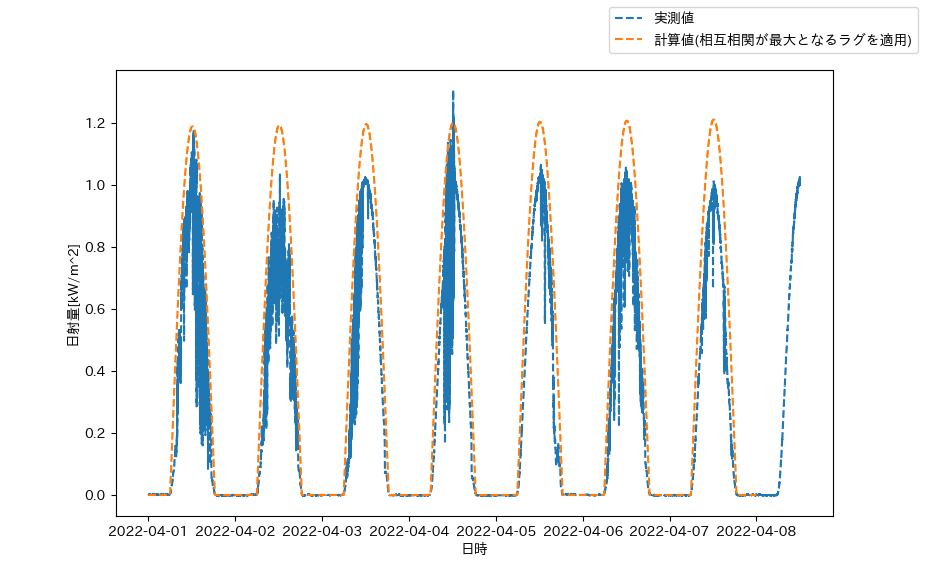
\includegraphics[width=160mm]{3.png}
    \caption{晴れの日の割合が大きい期間の実測データとラグを適用した計算値を重ねてプロットしたもの}
    \label{p3}
  \end{center}
\end{figure}


図\ref{p4}に図\ref{p2}と, 実測値より日時を750 \si{\second}遅らせた日射量の計算値を重ねてプロットしたものを示す.

\begin{figure}[H]
  \begin{center}
    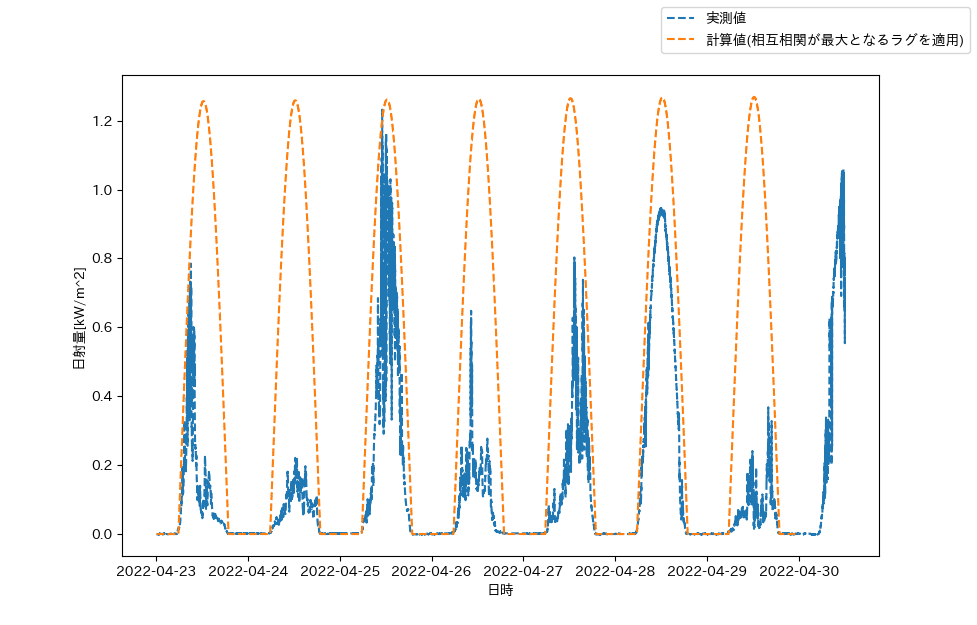
\includegraphics[width=160mm]{4.png}
    \caption{雨の日の割合が大きい期間の実測データとラグを適用した計算値を重ねてプロットしたもの}
    \label{p4}
  \end{center}
\end{figure}

\section{おわりに}
今回は, 晴れの日の割合が多い期間の実測データと, 雨の日の割合が多い期間の実測データのそれぞれに対して, 相互相関が最大となるラグの選定を行うことで, 実測データの概形と相互相関が最大となるラグの関係について調査した.
結果として, 日射量の計算値の概形に近い晴れの日の割合が多い期間の実測データを用いた時は, 実測値から日時を32 \si{\second}ずらしたときに相互相関が最大となったが, 雨の日の割合が多い期間の実測データを用いた時は, 実測値から日時を750 \si{\second}ずらしたときに相互相関が最大となり, 実測値の概形によって相互相関が最大となるラグの値が大きく変化することが分かった.
したがって, 相互相関を取るデータの吟味を今後行う.

\end{document}